\PassOptionsToPackage{dvipsnames}{xcolor}
\documentclass{beamer}
\usepackage{xcolor}
\usepackage{pgfpages}

\usepackage[style=authortitle]{biblatex}

\setbeameroption{show notes on second screen}

\usepackage[utf8]{inputenc}
\usepackage[T1]{fontenc}
\usepackage{lmodern}
\usepackage{fontawesome}

\usepackage{minted}

\usepackage{listings}

\usepackage[american]{babel}

\usepackage{
    amsmath,
    amsfonts,
    amssymb
}

\usepackage[os=win]{menukeys}

\usetheme{UOS}

\graphicspath{{img/}}

% use this with \begin{pythoncode} ... \end{pythoncode}
\newminted{python}{linenos=false}

\newminted[outputcode]{text}{linenos=false}

% this gets rid of red boxes around syntax errors in minted
\AtBeginEnvironment{minted}{%
  \renewcommand{\fcolorbox}[4][]{#4}}

% removes the prefix "Figure 1:" in figure captions
\setbeamertemplate{caption}{\raggedright\insertcaption\par}


\begin{document}

\title[Object Oriented Programming]{Week 9: Object Oriented Programming}
\subtitle{Basic Programming in Python}

\author[kgross, mpoemsl, sselbach]{Katharina Groß, Martin Pömsl, Sören Selbach}

\date{\today}

\begin{frame}[plain]
     \titlepage
\end{frame}

\begin{frame}
    \tableofcontents
\end{frame}

\section{Recap}

\subsection{Standard Library}

\begin{frame}{The Standard Library}

    Python's {\bf standard library} is a collection of modules included in most Python installations

    \begin{itemize}
        \item {\tt math}: mathematical functions
        \item {\tt random}: generate (pseudo-)random numbers
        \item {\tt copy}: create shallow and deep copies of objects
        \item {\tt time}: access the system's clock
        \item {\tt os} \& {\tt shutil}: operating system dependent actions like copying files, manipulating paths etc.
        \item {\tt sys}: technical things related to the Python interpreter, e.g. accessing command line arguments
    \end{itemize}

    \note{
        As always, there are many more, and they each have their own documentation:

        \vspace{1em}

        https://docs.python.org/3/library/
    }

\end{frame}

\subsection{Functions}

\begin{frame}[fragile]{Functions}

    \begin{block}{}
        {\bf Functions} are a way of organizing code such that it can be re-used easily
    \end{block}

    We give them data ({\bf arguments}), they do something with it and give back the result ({\bf return value})

    \vspace{1em}

    \begin{pythoncode}
    def compute_polynomial(x, c0, c1, c2, c3):
        y = c3 * x**3 + c2 * x**2 + c1 * x + c0

        return y

    poly_value = compute_polynomial(42, 4, 1, -3, -2.5)
    \end{pythoncode}

    \note{
        When a function is {\it defined} (with the {\tt def} keyword), none of the code is actually executed! We only define what happends when the function is {\tt called}. This can potentially be many times over the course of a program.
    }

\end{frame}

\section{Objects}

\begin{frame}[plain]
    \sectionpage
\end{frame}

\subsection{What is an Object?}

\begin{frame}{What is an Object?}

    \begin{block}{}
        An \textbf{object} is the \textbf{fundamental data structure} of Python
    \end{block}

    \begin{itemize}
        \item in Python, everything is an object:
        \begin{itemize}
            \item lists, tuples, dictionaries etc.
            \item strings
            \item ints, floats
            \item even functions!
        \end{itemize}
    \end{itemize}

\end{frame}

\begin{frame}[fragile]{Type}

    \begin{block}{}
        Every object belongs to a \textbf{type}
    \end{block}

    \vspace{1em}

    \begin{outputcode}
    >>> type([1, 2, 3])
    <class 'list'>

    >>> type(42)
    <class 'int'>

    >>> type(some_function)
    <class 'function'>
    \end{outputcode}

    \note{
        Objects always are {\it instances} of a class/type. There can be many instances of the same type - if you have three lists in your program, you have three instances of the type list.

        \vspace{1em}

        In Python, the term \textit{class} is mostly equivalent to \textit{type}. "What is the type of this object" is equivalent to "What is the class of this object".

        However, \textit{class} is mostly used when talking about \textit{user-defined} classes/types (more on that later), while \textit{type} is used when talking about \textit{built-in} types/classes.
    }

\end{frame}

\subsection{Attributes \& Methods}

\begin{frame}[fragile]{Attributes}

    \begin{block}{}
        An \textbf{attribute} is a variable that belongs to an object
    \end{block}

    \begin{pythoncode}
    from time import localtime

    print(type(localtime))
    # <class 'builtin_function_or_method'>

    time_now = localtime()
    print(type(time_now))
    # <class 'time.struct_time'>

    year_now = time_now.tm_year  # 2019
    month_now = time_now.tm_mon  # 6
    \end{pythoncode}

    \note{
        The \textbf{function} \texttt{localtime} returns an \textbf{object} of type \texttt{time.struct\_time}. This object is stored in the \textbf{variable} \texttt{time\_now} and has the \textbf{attributes} \texttt{tm\_year} and \texttt{tm\_month}.

        \vspace{1em}

        Attributes of an object can be accessed by writing \texttt{object\_name.attribute\_name}
    }

\end{frame}

\begin{frame}[fragile]{Attributes}

    \begin{pythoncode}
from time import localtime, sleep

time_1 = localtime()    # create first time object

sleep(2)                # wait 2 seconds

time_2 = localtime()    # this is a different object!

print(time_1.tm_sec)    # e.g. 21
print(time_2.tm_sec)    # 23
    \end{pythoncode}

    \note{
        In general, the attributes with the same name but of different objects have different values!
    }

\end{frame}

\begin{frame}[fragile]{Methods}

    \begin{block}{}
        A \textbf{method} is a function that belongs to an object
    \end{block}

    \begin{pythoncode}
    list_1 = [1, 2, 3]
    list_2 = [3, 4, 5]

    # call method append of object list_1
    list_1.append(42)

    # call method remove of object list_2
    list_2.remove(4)

    # list_1: [1, 2, 3, 42]
    # list_2: [3, 5]
    \end{pythoncode}

    \note{
        Just like attributes, methods know which object they belong to.
    }

\end{frame}

\subsection{Variables Revisited}

\begin{frame}[fragile]{Variables Revisited}

    So far, we have treated variables like \textbf{containers} that store \textbf{values} \\
    With this idea, we cannot explain this behavior:

    \vspace{1em}

    \begin{pythoncode}
    list_1 = [1, 2, 3]
    list_2 = list_1

    list_2.append(42)

    # list_1: [1, 2, 3, 42]
    # list_2: [1, 2, 3, 42]
    \end{pythoncode}

\end{frame}

\begin{frame}{Expectation}

    \begin{center}
        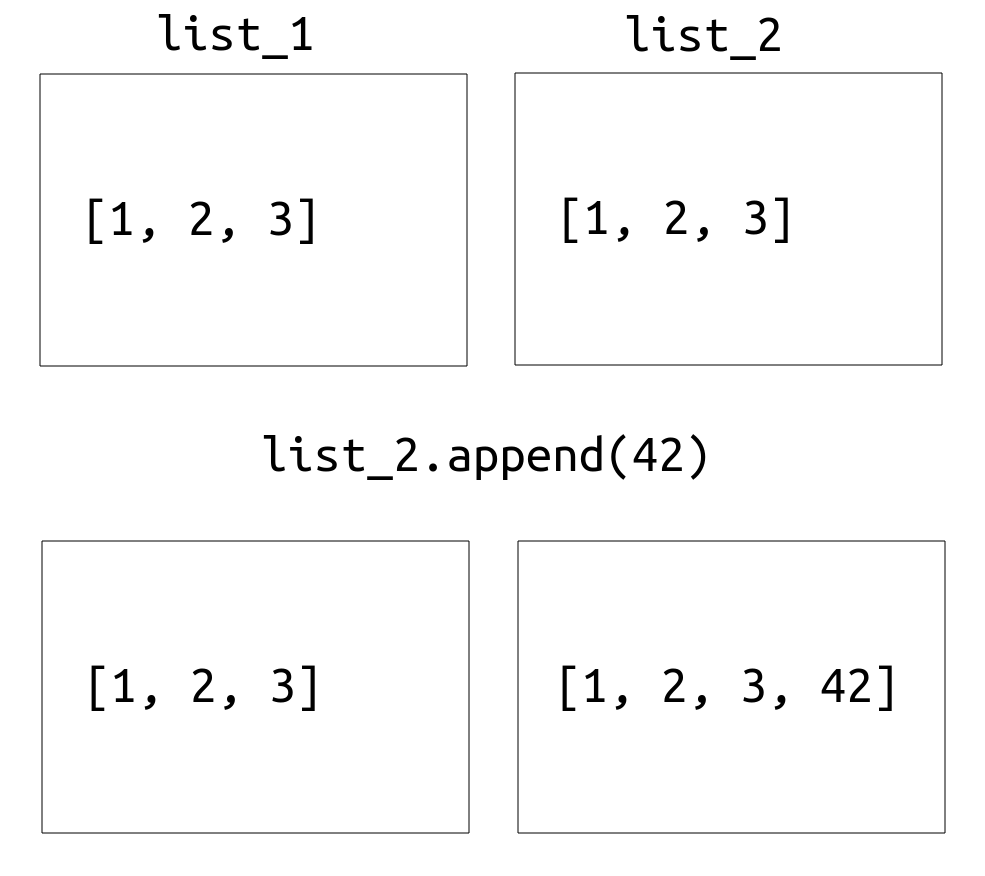
\includegraphics[height=0.8\textheight]{09_OOP/container_model.png}
    \end{center}

\end{frame}

\begin{frame}{Expectation}

    \begin{center}
        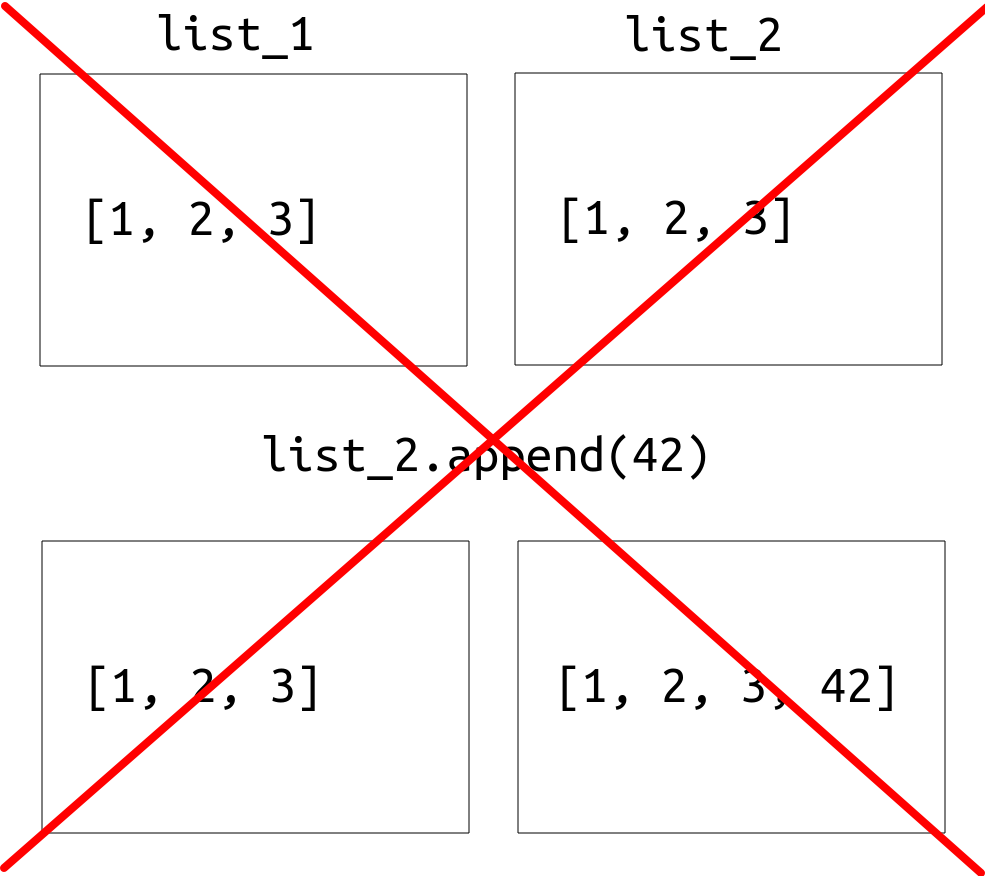
\includegraphics[height=0.8\textheight]{09_OOP/container_model_X.png}
    \end{center}

\end{frame}

\begin{frame}{Reality}

    \begin{block}{}
        Variables only contain \textbf{pointers} to objects!\\
        Multiple pointers can point to the \textbf{same} object.
    \end{block}

    \vspace{1em}

    \begin{center}
        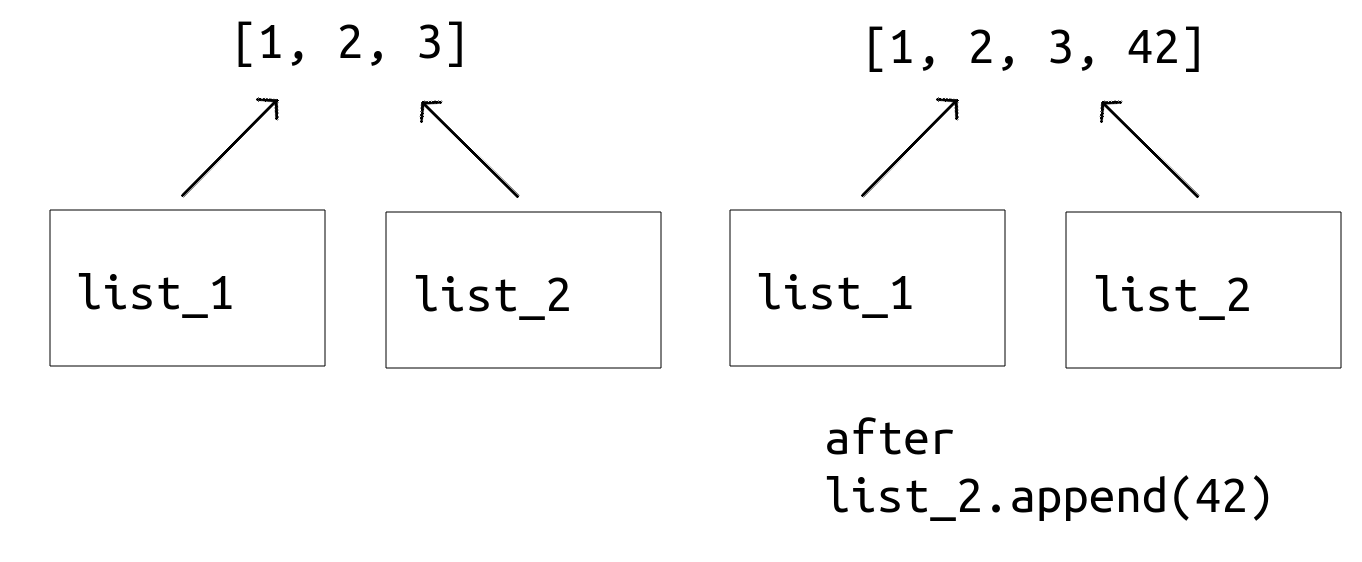
\includegraphics[width=\textwidth]{09_OOP/pointer_model.png}
    \end{center}

    \note{
        This means that the only thing that is stored "in" a variable is an address of an object that is somewhere else in the computer's memory.

        \vspace{1em}

        Note however, that if we create two identical lists like this:

        \vspace{1em}

        {\tt list\_1 = [1, 2, 3]} \\
        {\tt list\_2 = [1, 2, 3]}

        \vspace{1em}

        ... they are {\bf not} the same object! You can also use the {\tt copy} module to create copies of objects.

        \vspace{1em}

        This only makes a difference when working with \textit{mutable} objects such as lists or dictionaries.
    }

\end{frame}

\subsection{String Representation}

\begin{frame}{String Representation}

    Some object types have an intuitive way to display them as text:
    \begin{itemize}
        \item {\tt float}/{\tt int}: use decimal notation
        \item {\tt list}: use {\tt [element1, element2, ...]}
        \item {\tt time.struct\_time}: {\tt time.struct\_time(tm\_year=2019, tm\_mon=6, ...)}
    \end{itemize}

    Others do not. In this case, you get a generic string:
    \begin{itemize}
        \item {\tt <enumerate object at 0x7f38491d75a0>}
        \item {\tt <function test at 0x7f384941b400>}
    \end{itemize}

\end{frame}

\begin{frame}[fragile]{Example: Counter}

    The {\tt collections} module provides the class {\tt Counter}, which can count elements of lists, strings etc.:

    \vspace{1em}

    \begin{pythoncode}
    from collections import Counter

    some_string = "abccbcabcbcbbbabcbbbbab"

    char_counter = Counter(some_string)
    \end{pythoncode}

    \vspace{1em}

    Now we have an {\bf object} of type {\tt Counter}

\end{frame}

\begin{frame}[fragile]{Example: Counter}

    This {\tt Counter} object has methods we can access:

    \vspace{1em}

    \begin{pythoncode}
    from collections import Counter

    some_string = "abccbcabcbcbbbabcbbbbab"

    char_counter = Counter(some_string)

    print(char_counter.most_common(2))
    # [('b', 13), ('c', 6)]
    \end{pythoncode}

\end{frame}

\section{OOP}

\begin{frame}[plain]
    \sectionpage
\end{frame}

\subsection{Motivation}

\begin{frame}[fragile]{Object Oriented Programming}

    So far, we have been solving problems by writing a bunch of functions and feeding them with data

    For larger projects that require modularity, this can get quite cumbersome

    \begin{pythoncode}
def animate_legs_of_large_penguin(penguin_tom, time):
    # I don't want to do this
    \end{pythoncode}

    \begin{block}{}
        \textbf{Object Oriented Programming (OOP)} is a programming paradigm in which we design programs as {\it objects} that {\it interact} with each other
    \end{block}

    \note{
        Imagine we want to simulate a Zoo and want to visually animate the legs of all the animals. The logic for animating the legs of a Penguin is probably very different from animating the legs of an Elephant, and so we need different functions for that. \\

        \vspace{1em}

        The problem here lies in how we organize these functions. We could have very long and detailed names like {\tt animate\_legs\_of\_large\_penguin}, but this easily gets convoluted.

        \vspace{1em}

        OOP aims to give programs more structure by grouping semantically related pieces of data and methods into {\bf objects}.
    }

\end{frame}

\begin{frame}[fragile]{Object Oriented Programming}

    Suppose we want to simulate a Zoo

    \vspace{0.5em}

    Instead of writing many functions like

    \begin{itemize}
        \item {\tt animate\_legs\_of\_large\_penguin}
        \item {\tt animate\_legs\_of\_baby\_elephant}
        \item {\tt animate\_legs\_of\_giraffe}
    \end{itemize}

    \vspace{1em}

    We could have \textbf{object types} {\tt LargePenguin}, {\tt Giraffe} etc. that all have a \textbf{method} {\tt animate\_legs}

    \begin{pythoncode}
    tom = LargePenguin()
    tom.animate_legs(10)
    \end{pythoncode}

\end{frame}

\subsection{User-Defined Classes}

\begin{frame}[fragile]{User-Defined Classes}

    We need the ability to define our own \textbf{types}!

    \vspace{1em}

    \begin{pythoncode}
class LargePenguin:
    # functions defined in here are methods!

    def animate_legs(self, time):
        """animates legs of Penguin object for given time"""
        # ...

    def animate_wings(self, time):
        # ...
    \end{pythoncode}

    \vspace{1em}

    When a method is called, it automatically gets passed a pointer to the object it belongs to!

    \note{
        Note that the {\it naming convention} for user-defined classes is UpperCamelCase. Like functions, they also get their own {\bf docstring} at the very top!

        \vspace{1em}

        {\bf The Argument self:} Remember how we said in the beginning that a method {\it knows} which object it belongs to? This should be weird to you, because we only define {\bf one} method for {\bf all} LargePenguins. How can it know on {\bf which} LargePenguin it is called, as there could be many different instances?

        \vspace{1em}

        {\bf Answer:} When a method is called, it automatically gets passed a pointer to the object it belongs to! This is always the {\bf first positional argument}. By convention, this is almost always called {\tt self}, and it needs to be accepted in every (normal) method! We say a method is {\bf bound} to an object.
    }

\end{frame}

\begin{frame}[fragile]{User-Defined Classes}

    What about attributes? They can be defined similarly to variables:

    \vspace{1em}

    \begin{pythoncode}
    # create LargePenguin object
    tom = LargePenguin()

    # give it the attribute 'age'
    tom.age = 11
    tom.fav_food = "fish"
    \end{pythoncode}

    \vspace{1em}

    99\% of the time we want to define attributes {\bf immediately after we create the object}

\end{frame}

\begin{frame}[fragile]{The Constructor}

    \begin{block}{}
        The {\bf constructor} of a class is a \textit{special method} that gets called when a \textbf{new instance} of that class is created
    \end{block}

    \begin{pythoncode}
class LargePenguin:
    def __init__(self, age, fav_food):
        self.age = age
        self.fav_food = fav_food

    def animate_legs(self, time):
        # ...

tom = LargePenguin(age=11, fav_food="fish")
timothy = LargePenguin(age=6, fav_food="steak")
    \end{pythoncode}

    \note{
        The constructor {\bf must} be named {\tt \_\_init\_\_(self, ...)}!

        \vspace{1em}

        Now {\tt tom} is a {\tt LargePenguin} object with attributes {\tt tom.age == 11} and {\tt tom.fav\_food == "fish"}. {\tt timothy} is also a {\tt LargePenguin} object, but has attributes {\tt timothy.age == 6} and {\tt timothy.fav\_food == "steak"}. Both have the method {\tt animate\_legs}.
    }

\end{frame}

\begin{frame}{Dunder Methods}

    The constructor is part of a family of special methods, called dunder-methods (double underscore)

    \vspace{1em}

    They all do special things, depending on their name:
    \begin{itemize}
        \item {\tt \_\_init\_\_}: contructor - gets called on object creation
        \item {\tt \_\_str\_\_}: defines how objects of this type are converted to strings
        \item {\tt \_\_add\_\_}: defines how objects of this type work with the "{\tt +}" operator
    \end{itemize}

    \vspace{1em}

    There are of course many, many more.

    \note{
        Because they affect the program without ever being explicitly called, dunder-methods are also often called {\it magic methods}.

        \vspace{1em}

        Here you can find a complete list of all definable dunder-methods: \\
        https://docs.python.org/3/reference/datamodel.html\#special-method-names
    }

\end{frame}

\begin{frame}[fragile]{{\tt \_\_str\_\_}}

    \begin{block}{}
        {\tt \_\_str\_\_} changes how an object is displayed as a string
    \end{block}

    \begin{pythoncode}
class LargePenguin:
    # ...

    def __str__(self):
        s = "A penguin that is {} years old and likes {}"
        return s.format(self.age, self.fav_food)

    # ...

tom = LargePenguin(age=11, fav_food="fish")
print(tom)
    \end{pythoncode}

\end{frame}

\begin{frame}[fragile]{{\tt \_\_str\_\_}}

    {\bf Output without {\tt \_\_str\_\_}:}

    \vspace{1em}

    \begin{outputcode}
  <__main__.LargePenguin object at 0x7f384abebbe0>
    \end{outputcode}

    \vspace{2em}

    {\bf Output with {\tt \_\_str\_\_}:}

    \vspace{1em}

    \begin{outputcode}
  A penguin that is 11 years old and likes fish
    \end{outputcode}

\end{frame}

\begin{frame}[fragile]{Private Attributes}

    Sometimes we want to have {\bf private} attributes (i.e. ones that are only accessible by the object they belong to)

    \vspace{1em}

    {\it This does not exist in Python.}

    \vspace{1em}

    Instead, this is handled by yet another {\bf convention}:

    \vspace{1em}

    \begin{pythoncode}
class MyClass:
    def __init__(self):
        # this is marked as private with the _
        self._some_attr = 42
    \end{pythoncode}

\end{frame}

\subsection{Properties}

\begin{frame}[fragile]{Properties}

    Sometimes we want to have {\bf read-only attributes} (i.e. ones that can be accessed from anywhere, but cannot be changed)

    \vspace{1em}

    These are called {\bf properties}. One way of achieving this is using a method:

    \begin{pythoncode}
    class MyClass:
        def my_property(self):
            return 42

    my_object = MyClass()
    print(my_object.my_property())  # 42
    \end{pythoncode}

    However, unlike normal attributes we have to write {\tt ()}

\end{frame}

\begin{frame}[fragile]{Properties}

    Writing {\tt @property} before a method definition makes it so that it is accessible like an attribute:

    \vspace{1em}

    \begin{pythoncode}
    class MyClass:
        @property
        def my_property(self):
            return 42

    my_object = MyClass()
    print(my_object.my_property)  # 42
    \end{pythoncode}

    \note{
        {\tt @property} is a {\bf decorator}. Decorators modify the behavior of functions and methods. Again, there are more predefined ones, and you can define your own. We will not go into when and how to use them, as we don't have the time for that, but if you are running out of new things to learn, they can be useful.

        \vspace{1em}

        http://book.pythontips.com/en/latest/decorators.html
    }

\end{frame}

\begin{frame}[fragile]{Properties}

    {\tt @property} is often used together with "private" attributes:

    \vspace{1em}

    \begin{pythoncode}
    class MyClass:
        def __init__(self):
            self._some_hidden_attr = 42

        @property
        def some_attr(self):
            return self._some_hidden_attr
    \end{pythoncode}

    \vspace{1em}

    Now we have an attribute that from the outside can only be read, but can be changed from the inside by modifying {\tt \_some\_hidden\_attr}

    \note{
        Again, note that technically, you still {\bf can} change {\tt \_some\_hidden\_attr} from the outside - but you really should not. Whenever you are using {\tt some\_object.\_some\_property} that starts with an \_, you are using someone's code in an unintended way, which has the potential to break things.
    }

\end{frame}

\begin{frame}[fragile]{Properties}

    \begin{outputcode}
    >>> my_object = MyClass()
    >>> my_object.some_attr
    42
    >>> my_object.some_attr = 43
    Traceback (most recent call last):
      File "<stdin>", line 1, in <module>
    AttributeError: can't set attribute
\end{outputcode}

\end{frame}

\subsection{Inheritance}

\begin{frame}{Inheritance}

    Suppose you have a class {\tt Bird} and want to create another class {\tt Penguin} that only differs in some points.

    \vspace{1em}

    \begin{block}{}
        A class can \textbf{inherit} from another class, i.e. it adopts all attributes and methods of it. It can then overwrite existing methods and define new ones.
    \end{block}

    The class that inherits is called {\bf child} or {\bf subclass}

    \vspace{1em}

    The class that is inherited from is called {\bf parent}, {\bf superclass} or {\bf base class}

    \note{
        Think of inheritance as making some concept more specialized. Think of the base class {\tt Phone}, which has a method {\tt call}. A {\tt SmartPhone} inherits from {\tt Phone} because it is a specialized version of a phone. It might have the method {\tt send\_message} in addition. An old {\tt RotaryPhone} also inherits from {\tt Phone}, but does not inherit from {\tt SmartPhone}.

        \vspace{1em}

        In Python, everything automatically inherits from {\tt object}. {\it Exceptions} are another nice example: Every Exception inherits from {\tt BaseException}, i.e. {\tt SyntaxError}. {\tt IndentationError} in turn inherits from {\tt SyntaxError}. Here is the hierarchy again:

        \vspace{1em}

        https://docs.python.org/3/library/exceptions.html\#exception-hierarchy
    }

\end{frame}

\begin{frame}[fragile]{Inheritance}

    \begin{pythoncode}
    class Bird:
        def walk(self, distance):
            # code for walking

        def fly(self, distance):
            # code for flying

    class Penguin(Bird):
        def waddle(self, distance):
            # code for waddling

        fly = None
    \end{pythoncode}

    \note{
        {\tt Penguin} inherits from {\tt Bird}, which means it gets the methods {\tt walk} and {\tt fly} without having to re-implement them. Now there are two things going on:
        \begin{enumerate}
            \item Penguins can waddle, while normal birds cannot, and so we add the method {\tt waddle}.
            \item Penguins cannot fly, and so we overwrite the method {\tt fly}. There are a couple of ways for doing this - we could for instance re-define it in {\tt Penguin} and have it do nothing. The convention is to just set the entire method to {\tt None} (so it is not even a method afterwards). This way, when you try to call {\tt some\_penguin.fly(10)} you get a {\tt TypeError}
        \end{enumerate}
    }

\end{frame}

\begin{frame}[fragile]{Accessing the Superclass}

    Suppose we want to create a class {\tt AwesomePenguin} that waddles twice as far as a normal one would.

    \begin{block}{}
        {\tt super()} lets us access the superclass we inherit from. Note that again, self is automatically provided.
    \end{block}

    \begin{pythoncode}
    class AwesomePenguin(Penguin):
        def waddle(self, distance):
            super().waddle(distance)
            super().waddle(distance)
    \end{pythoncode}

\end{frame}

\begin{frame}[fragile]{Inheriting Attributes}

    {\bf Attributes} are inherited by default, because we inherit the {\bf constructor}. If we want to add some, we need to overwrite it:

    \vspace{0.7em}

    \begin{pythoncode}
class SuperClass:
    def __init__(self):
        self.attr_1 = 42

class SubClass(SuperClass):
    def __init__(self):
        # call superclass constructor
        # to keep its attributes
        super().__init__()

        self.attr_2 = "important stuff"
    \end{pythoncode}

\end{frame}

\begin{frame}{Reading}

    This is a good (and rather short) article to recap your understanding of objects and types in Python:

    \vspace{1em}

    \url{https://eli.thegreenplace.net/2012/03/30/python-objects-types-classes-and-instances-a-glossary}

\end{frame}

\section{Homework}

\begin{frame}[plain]
    \sectionpage
\end{frame}


\end{document}
